%\documentclass{article}
%
%\usepackage{NotesPackage}
%
%\usepackage[version=4]{mhchem}
%\usepackage{caption}
%\captionsetup{justification=centering}
%
%\DeclareMathOperator{\sgn}{sgn}
%
%\author{Willoughby Seago}
%\date{14 January, 2020}
%\title{Physics of Matter}
%
%\begin{document}
%    \maketitle
%    \tableofcontents
    
    \part{Solids}
    \section{Pair Potentials}
    Any two atoms experience a pair potential.
    Wherever this pair potential is at a minimum the atoms are in a stable configuration.
    One such stable configuration occurs at distances on the order of \SI{e-10}{m} as in chemical bonds.
    This is the main region of interest for solids.
    One of the most common pair potential models is the Lennard--Jones potential
    \[U(r) = 4\epsilon\left[\left(\frac{\sigma}{r}\right)^{12} - \left(\frac{\sigma}{r}\right)^6\right]\]
    The equilibrium point, \(r_0\), occurs when the forces balance.
    The force is given by
    \[F = -\dv{U}{r} = 4\epsilon\left[-12\frac{\sigma^{12}}{r^{13}} + 6\frac{\sigma^6}{r^7}\right]\]
    \[F(r_0) = 0 \implies r_0 = 2^{1/6}\sigma\]
    \[U(r_0) = -\epsilon\]
    so the depth of the potential well is \(\epsilon\).
    For argon atoms \(\epsilon = \SI{0.01}{eV}\) and \(\sigma = \SI{3.4}{\angstrom}\).
    So even a low temperature \(T\approx\SI{100}{K}\), or \(k_BT\approx\epsilon\) is enough to disrupt bonding.
    This is seen in the low boiling point of argon at \SI{87}{K}.
    
    \subsection{Ionic Bonding}
    Ionic bonding is the attraction via electron exchange to produce filled orbitals that then results in oppositely charged particles that attract each other through Coulomb forces.
    Assuming only one electron is exchanged the attractive Coulomb force has a potential energy of
    \[U_C = \pm\frac{1}{4\pi\varepsilon_0}\frac{e^2}{r}\]
    where the \(\pm\) accounts for the possible pairings of positive and negative charge.
    There is also a repulsive term determined experimentally as
    \[U_R = \frac{A}{r^9}\]
    for some constant \(A\).
    The total potential is then
    \[U = U_C + U_R = \pm\frac{1}{4\pi\varepsilon_0}\frac{e^2}{r} + \frac{A}{r^9}\]
    This system can only be at equilibrium for a negative Coulomb potential, when this is the case the equilibrium position is
    \[F = -\dv{U}{r} = 0\]
    \[\frac{1}{4\pi\varepsilon_0}\frac{e^2}{r_0^2} - \frac{9A}{r_0^10} = 0\]
    hence
    \[A = \frac{1}{9}\frac{e^2}{4\pi\varepsilon_0}r_0^8\]
    \[U = \frac{e^2}{4\pi\varepsilon_0}\left[\pm\frac{1}{r} + \frac{r_0^8}{9r^9}\right]\]
    The depth of the potential well for a pair of dissimilar charges is
    \[U(r_0) = -\frac{e^2}{4\pi\varepsilon_0}\frac{8}{9}\frac{1}{r_0}\]
    This can be written in a form analogous to the Lennard--Jones potential:
    \[U = \epsilon^*\left[\pm\left(\frac{\sigma}{r}\right)^1 + \left(\frac{\sigma}{r}\right)^9\right]\]
    We find that the minimum occurs at \(r_0 = 9^{1/8}\sigma\) and at this distance we get
    \[U(r_0) = \epsilon^*\left[9^{-9/8} - 9^{-1/8}\right]\]
    giving
    \begin{equation}\label{eqn:ionic potential}
        U = 1.481\epsilon\left[\pm\left(\frac{\sigma}{r}\right)^1 + \left(\frac{\sigma}{r}\right)^9\right]
    \end{equation}
    where \(\epsilon\) is the binding energy.
    
    This is an ionic pair potential.
    For \ce{NaCl} molecules \(\epsilon = \SI{5.32}{eV}\) and \(\sigma = \SI{1.83}{\angstrom}\).
    This is about 500 times stronger bonding energy than between argon molecules.
    
    \subsection{Other Bonds}
    A pair potential like this can only be defined for van der Waal's forces and ionic bonds other types of bond don't have such a nice potential.
    
    Covalent bonds occur when electrons are shared between two or more atoms.
    Because it relies so heavily on the aim of gaining a full subshell it requires quantum mechanics to explain the potential so is beyond the scope of the course.
    
    Metallic bonding occurs when electrons are denoted to a sea of delocalised electrons which then acts like glue between molecules.
    Again to find the potential we require quantum mechanics.
    
    Hydrogen bonding occurs when a hydrogen atom forms a covalent bond with a highly electronegative element (\ce{O}, \ce{N}, \ce{F}) and since Hydrogen has only one electron this exposes the nucleus (which is just a proton) which leaves part of the molecule slightly positively charged allowing for a Coulomb potential with another negative molecule.
    Hydrogen bonds are the reason for water's high surface tension.
    
    \subsection{Solid Characteristics}
    \begin{itemize}
        \item Exist in a vacuum - solids require no external forces to pack the particles together as the bonds are strong enough to do this themselves.
        Liquids on the other hand need a pressure greater than that at the triple point to exist.
        \item Ubiquitous - solids occur in almost all materials at low enough temperatures.
        \item Strength - solids can withstand a shear stress, unlike fluids.
        \item Melting and sublimation - the melting and sublimation points of solids depend on the strength of the bonds, stronger bonds will hold together at higher temperatures
        \item Order - solids, especially crystals, have long range structure.
    \end{itemize}
    
    \subsection{Crystals}
    Apart from a few exceptions the lowest energy state of matter, which is what will form at the lowest temperatures, is a crystalline solid.
    Diffraction studies show that crystals have long range order; they form a regular array over macroscopic distances.
    Recall the radial distribution function that was derived for fluids, it also describes solids well but \(g(r)\) and \(\rho(r)\) will be different to a liquid.
    \[\dd N(r) = \rho(r)4\pi r^2\dd r = \expected{\rho}g(r)4\pi r^2\dd r\]
    For a solid because of the long range structure \(g(r)\) is zero at most values of \(r\) and then forms sharp peaks at specific values of \(r\).
    Where these peaks occur depends on the crystal structure.
    Since the order is long range \(g(r)\) doesn't tend to a particular value as it did for disordered matter.
    
    Crystals are described by a lattice and a basis.
    A crystal lattice is an infinite grid of identical points representing the repetition of the structure.
    We will start with the way we describe the lattice.
    It can be described by three vectors \(\vv a\), \(\vv b\) and \(\vv c\) and the angles between them.
    These three vectors make up a (normally not orthonormal) basis set that spans the lattice.
    The lattice is then given as the set of all vectors \(\vv R = n_1\vv a + n_2\vv b + n_3\vv c\) where \(n_i\in\bb Z\).
    A unit cell is a what you get if you take the basis vectors as the edges of a volume.
    Each unit cell contains at least one lattice point.
    Note that a lattice point can be shared between multiple unit cells.
    In this case it contributes only part of a lattice point to each.
    For example the corner of a unit cell is also the corner of seven other unit cells so only contributes \(1/8\)th of a lattice point to each unit cell.
    A lattice point on the face of a unit cell is in two unit cells so contributes half a lattice point to each.
    
    There can be multiple, equally valid, unit cells (and hence basis vectors) for each crystal structure.
    It is always possible to find a unit cell that contains exactly one lattice point.
    This is known as the primitive unit cell.
    It isn't necessarily useful as it may be less regular than a larger unit cell and so harder to work with.
    The cells can be described by where in them there are lattice points (other than the corners) and their shapes.
    For example a lattice point in the centre of a unit cell makes it a body--centred unit cell, one lattice point on the face of the unit cell makes it one--face--centred (note that there will be half a lattice point on one face and half on the opposite face) and one lattice point in the middle of each face makes it face--centred.
    
    The lengths of the basis vectors/edges of the unit cell are \(a\), \(b\) and \(c\).
    Denoting the angle between two vectors \(\vv x\) and \(\vv y\) as \(\vv x\angle\vv y\) we get \(\vv a\angle\vv b = \gamma\), \(\vv a\angle\vv c = \beta\) and \(\vv b\angle\vv c = \alpha\).
    Combined \(a\), \(b\), \(c\), \(\alpha\), \(\beta\) and \(\gamma\) are known as the lattice parameters or cell dimensions.
    
    The basis of a crystal is a list of all atoms in the unit cell and their positions in terms of the basis vectors.
    The point \(\vv P = x\vv a + y\vv b + z\vv c\) is usually given as \((x, y, z)\).
    For a simple cubic structure there is one basis point on every single corner.
    This gives a basis of \((0, 0, 0)\) for the unit cell since each corner of the unit cell is at the origin of one unit cell so we only need to specify that there is an atom at the origin.
    A body centred basis is the same as simple cubic but with a basis point in the centre so its basis is \((0, 0, 0)\) and \((1/2, 1/2, 1/2)\).
    One--face--centred has a basis \((0, 0, 0)\) and \((1/2, 1/2, 0)\).
    Face--centred has a basis \((0, 0, 0)\), \((1/2, 1/2, 0)\), \((1/2, 0, 1/2)\) and \((0, 1/2, 1/2)\).
    
    Note that the lattice points all have to have the same type of atom at the corner if there is more than one type of atom.
    
    \section{Crystal Structure}
    \subsection{The Seven Unit Cells}
    There are seven fundamentally different unit cells.
    They can be distinguished by so the side lengths and angles relate to each other.
    \begin{itemize}
        \item Cubic - \(a = b = c\) and \(\alpha = \beta = \gamma = \SI{90}{\SIUnitSymbolDegree}\) - It is a cube
        \item Tetragonal - \(a = b \ne c\) and \(\alpha = \beta = \gamma = \SI{90}{\SIUnitSymbolDegree}\) - Cube stretched in one direction
        \item Orthorhombic - \(a \ne b \ne c\) and \(\alpha = \beta = \gamma = \SI{90}{\SIUnitSymbolDegree}\) - Cuboid
        \item Monoclinic - \(a \ne b \ne c\) and \(\alpha = \gamma = \SI{90}{\SIUnitSymbolDegree}\) and \(\beta \ne \SI{90}{\SIUnitSymbolDegree}\) - Cuboid pushed over
        \item Hexagonal - \(a = b \ne c\) and \(\alpha = \beta = \SI{90}{\SIUnitSymbolDegree}\) and \(\gamma = \SI{120}{\SIUnitSymbolDegree}\) - Three of these share an edge and the resulting shape has a hexagonal cross section
        \item Trigonal - \(a = b = c\) and \(\alpha = \beta = \gamma \ne \SI{120}{\SIUnitSymbolDegree}\) - Cube pushed over
        \item Triclinic - \(a \ne b \ne c\) and all angles different and not \SI{90}{\SIUnitSymbolDegree} - as irregular as possible
    \end{itemize}
    In this course we are mostly interested in the two simplest, cubic and tetragonal, and the face/body--centred versions of these.
    
    \begin{figure}[ht]
        \centering
        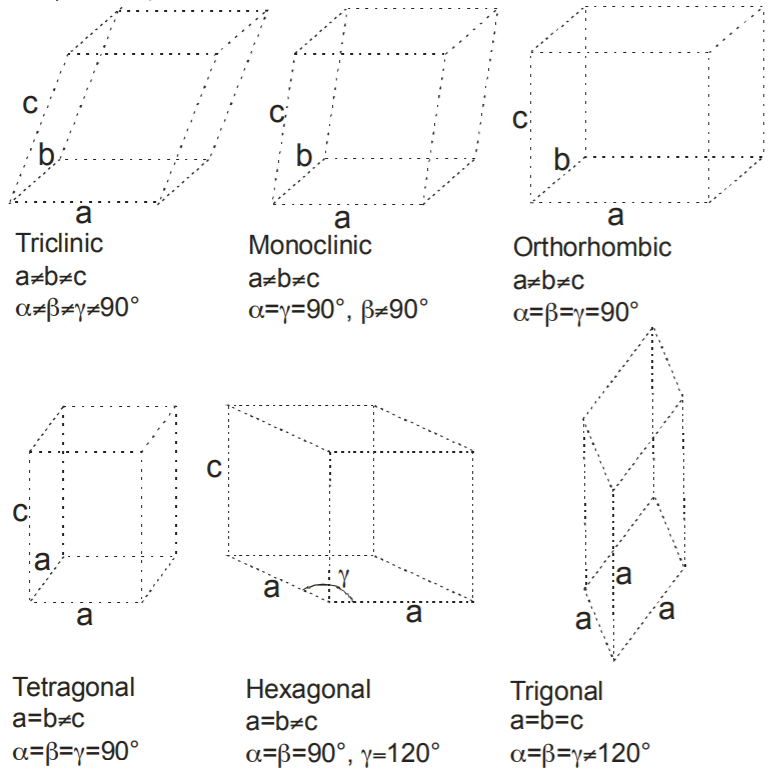
\includegraphics[scale=0.3]{crystal_structures.png}
        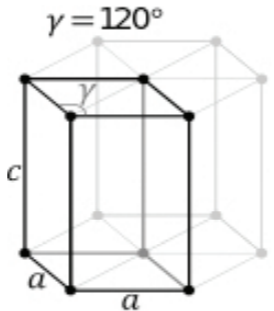
\includegraphics[scale=0.7]{hexagonal.png}
        \caption{The different crystal structures and the reason hexagonal is called hexagonal}
    \end{figure}
    
    \subsection{Planes}
    Planes in a crystal are defined by their Miller indices, \((hkl)\).
    These planes are actually sets of equally spaced, parallel, planes.
    To find the Miller indices we take the plane closest to the origin that doesn't contain the origin and we look at where it intercepts the unit cell axes.
    The plane with Miller indices \((hkl)\) intercepts the \(x\) axis at \(a/h\), the \(y\) axis at \(b/k\) and the \(z\) axis at \(c/l\).
    This value of \((hkl)\) then describes any set of parallel planes to this which are then called the \((hkl)\) planes.
    If a plane is parallel to an axis then it intercepts that axis at infinity so the corresponding index is 0.
    If the plane cuts the axis on the negative side of the origin then the relevant Miller index is negative which is usually denoted with a bar such as \((1\bar 1 0)\) is the set of planes parallel to the plane which crosses the \(x\) axis at \(a\), the \(y\) axis at \(-b\) and is parallel to the \(z\) axis.
    
    We consider a plane through the origin and the nearest parallel plane.
    The distance between the planes is \(d(hkl)\) often abbreviated \(d\)  if there is only one set of planes in consideration.
    Define the angle from the \(x\), \(y\) and \(z\) axis to the perpendicular to the plane as \(\psi_1\), \(\psi_2\) and \(\psi_3\) respectively.
    Since the planes are parallel the normal to the planes is the shortest distance between them.
    We find that
    \[d = \frac{a}{h}\cos\psi_1 = \frac{b}{k}\cos\psi_2 = \frac{c}{l}\cos\psi_3\]
    In the case where \(\alpha = \beta = \gamma = 90\SIUnitSymbolDegree\) we get that
    \[\cos^2\psi_1 + \cos^2\psi_2 + \cos^2\psi_3 = 1\]
    so
    \[\frac{1}{d^2} = \frac{h^2}{a^2} + \frac{k^2}{b^2} + \frac{l^2}{c^2}\]
    for a cubic cell this simplifies to
    \begin{equation}\label{eqn:d(hkl)}
        d = \frac{a}{\sqrt{h^2 + k^2 + l^2}}
    \end{equation}
    
    A set of lattice planes is referred to with brackets as \((hkl)\).
    When this set is identical to another by virtue of symmetry the two sets are equivalent and belong to a family, referred to using curly brackets as \(\{hkl\}\).
    
    The planes parallel to \((hkl)\) on the opposite side of the origin, that is \((\bar h\bar k\bar l)\) are always equivalent to \((hkl)\).
    After this the planes that are equivalent depend on the symmetry of the crystal.
    For the least symmetric crystal unit cell (triclinic) the only equivalent planes are \((hkl)\) and \((\bar h\bar k\bar l)\).
    For the most symmetric crystal unit cell (cubic) all possible arrangements of \(h\), \(k\) and \(l\) and their negatives are equivalent so for distinct \(h\), \(k\) and \(l\) there are 24 equivalent ways to describe \((hkl)\).
    
    Directions in the unit cell are denoted with square brackets as \([hkl]\) for a specific direction or with angle brackets \(\langle hkl\rangle\) for a family.
    For a cubic lattice these are perpendicular to the corresponding planes \((hkl)\) or \(\{hkl\}\).
    
    \subsection{Counting Particles and Density}
    The number of particles in a unit cell is given by the sum of the particles partly in the unit cell weighted by how much of the particle is in the unit cell.
    This means that if a particle is only half in the unit cell it only counts as half a particle.
    It is often convenient to think of the particles as spheres with the largest radius possible so that they don't overlap.
    If the number of particles in the unit cell is \(N_p\) and the particles have mass \(M_p\) and the unit cell has volume \(V_{UC}\) then the density of the solid is
    \[\rho = \frac{N_pM_p}{V_{UC}}\]
    If there is more than one type of particle then this extends to
    \[\rho = \frac{1}{V_{UC}}\sum_i N_{pi}M_{pi}\]
    where \(N_{pi}\) is the number of particles of the \(i^\text{th}\) type of particle and \(M_{pi}\) is the mass of the \(i^\text{th}\) type of particle.
    
    \subsection{Coordination and Packing}
    The coordination of a particle is the number of nearest neighbours that it has in a given crystal structure.
    The nearest neighbours are the particles that are the minimum distance from the particle.
    In a crystal the coordination of a particle is an integer and the nearest neighbours are at a set distance.
    
    Different crystal structures have different efficiencies when it comes to fitting in particles into a set volume.
    One measure of efficiency is the packing fraction which is the fraction of space that is occupied by hard spheres of maximum radius in place of the particles.
    If the volume of the unit cell is \(V_{UC}\), the number of particles in the unit cell is \(N_p\) and the volume of one of the hard spheres is \(V_p\) then the packing fraction \(PF\) is given by
    \[PF = \frac{N_pV_p}{V_{UC}}\]
    The fraction of open space is then \(1 - PF\).
    
    The packing fraction and coordination number are both higher for denser lattices.
    When maximised the structure is said to be close packed.
    For a one component crystal face centred cubic lattices are close packed and so are hexagonal close packed lattices.
    These have a maximum packing fraction of \(PF \approx 0.74\) and coordination number of \(CN = 12\).
    
    \subsection{Typical Crystal Structures}
    \subsubsection{Simple or Primitive Cubic (sc)}
    One atom at each corner of a cubic lattice.
    Each atom has coordination number \(CN = 6\) and packing fraction \(PF = 0.524\).
    \subsubsection{Body Centred Cubic (bcc)}
    One atom at each corner of a cubic lattice and one in the centre of the lattice.
    Each atom has coordination number \(CN = 8\) and packing fraction \(PF = 0.68\).
    \subsubsection{Face Centred Cubic (fcc)}
    One atom at each corner of a cubic lattice and one atom in the centre of each face of the lattice.
    Each atom has coordination number \(CN = 12\) and packing fraction \(PF = 0.74\).
    
    The reason that both fcc (also known as cubic close packed) and hexagonal close packed are both close packed is that by moving layers of atoms it is possible to move from one to the other without changing the density.
    
    \section{Lattice Energy and Diffraction}
    We used pair potentials earlier to describe boding effects in a pair of free particles such as a diatomic molecule.
    For \(N\) interacting particles the total potential, \(U_T\), is the sum of the pair potentials \(U(r_{ij})\) where \(r_{ij}\) is the distance between the \(i^\text{th}\) and \(j^\text{th}\) atoms.
    Note the factor of \(1/2\) that stops double counting:
    \[U_T = \frac{1}{2}\sum_{i\ne j}U(r_{ij}) = \sum_{i>j}U(r_{ij})\]
    
    If this is a gas then as it becomes denser or becomes a liquid then the total potential becomes very complicated and would be best defined by a computer simulation.
    For a crystal however the structure allows for a well defined set of distances for each set of nearest neighbours.
    Even for an ideal crystal where there is an infinite number of particles since pair potentials generally scale as \(1/r^x\) we can often ignore the terms from particles more than a certain distance away.
    
    We expect that \(U_T\) will have a solution in the case of an infinite crystal and wit a goal to find it we rewrite \(U_T\) as a sum over increasing radial distance about the \(j^\text{th}\) particle with the distance from this particle being denoted \(r_i\) and the number of nearest neighbours at this distance being \(N_i\).
    Then
    \[U_T^j = \sum_{i = 1}^\infty N_iU(r_i)\]
    Converting this to a quantity per mole we get the total potential is
    \[U_T = \frac{1}{2}\sum_{j = 1}^{N_A}U_T^j\]
    we get the potential is
    \[U_T = \frac{1}{2}N_A\sum_{i = 1}^\infty N_iU(r_i)\]
    where again the factor of \(1/2\) stops double counting.
    This is the lattice energy or lattice potential and the sum is a lattice sum.
    
    \subsection{Van der Waals Solid}
    A van der Waals solid has a pair potential given by the Lennard--Jones potential:
    \[U(r) = 4\epsilon\left[\left(\frac{\sigma}{r}\right)^{12} - \left(\frac{\sigma}{r}\right)^6\right]\]
    where the lone pair separation is \(r_0 = 1.12\sigma\) and the potential well depth is \(\epsilon\).
    \begin{table}[ht]
        \centering
        \begin{tabular}{c|ccc}\hline
            \(i\) & \(r_i(a)\) & \(r_i(r_1)\) & \(N_i\)\\\hline
            1 & \(a/\sqrt{2}\) & \(r_1\) & 12\\
            2 & \(a\) & \(r_1\sqrt{2}\) & 6\\
            3 & \(a\sqrt{3/2}\) & \(r_1\sqrt{3}\) & 24\\
            4 & \(a\sqrt{2}\) & \(r_1\sqrt{4}\) & 12\\
            5 & \(a\sqrt{5/2}\) & \(r_1\sqrt{5}\) & 24\\
            6 & \(a\sqrt{3}\) & \(r_1\sqrt{6}\) & 8\\
            \(\vdots\) & \(\vdots\) & \(\vdots\) & \(\vdots\)\\\hline
        \end{tabular}
        \caption{The first six nearest neighbours for a face centred cubic crystal. The distance to the nearest neighbour is given in terms of the lattice parameter, \(a\), and the distance to the first nearest neighbour, \(r_1\).}
        \label{tab:fcc nn}
    \end{table}
    When calculating \(U_T\) we can safely assume that the very short range repulsive force is only important for the first nearest neighbour.
    For the values given in table \ref{tab:fcc nn} the lattice potential for a fcc crystal is
    \begin{align*}
        U_T &= \frac{N_A}{2}4\epsilon\left[12\left(\frac{\sigma}{r_1}\right)^{12} - 12\left(\frac{\sigma}{r_1}\right)^6 - 6\left(\frac{\sigma}{r_1\sqrt{2}}\right)^6 - 24\left(\frac{\sigma}{r_1\sqrt{3}}\right)^6\right. \\ &\hphantom{U_T = \frac{N_A}{2}4\epsilon}\left.-12\left(\frac{\sigma}{r_1\sqrt{4}}\right)^6 - 24\left(\frac{\sigma}{r_1\sqrt{5}}\right)^6 - 8\left(\frac{\sigma}{r_1\sqrt{6}}\right)^6 - \dotsb\right]\\
        &= 2\epsilon N_A\left[12\left(\frac{\sigma}{r_1}\right)^{12} - \left(\frac{\sigma}{r_1}\right)^6(12.0 + 0.750 + 0.888 + 0.188 + 0.192 + 0.037 +\dotsb)\right]
    \end{align*}
    Noting that the series is rapidly decreasing we ignore further terms to get
    \[U_T \lesssim 2\epsilon N_A \left[12\left(\frac{\sigma}{r_1}\right)^{12} - 14.05\left(\frac{\sigma}{r_1}\right)^6\right]\]
    where \(\lesssim\) indicates that further terms would reduce \(U_T\) but not by much.
    Evaluating for
    \[F = -\dv{U}{r} = 0\]
    we find that the equilibrium first nearest neighbour distance is \(r_1\lesssim 1.09\sigma\) which is about \(\SI{3}{\%}\) less than the free pair solution of \(r_0 = 1.12\sigma\).
    So we find that condensation to a solid causes bond lengths to contract.
    Each atom is now feeling the attractive force of more atoms.
    The depth of the potential well for each ion is \(U_T/N_A = 8.2\epsilon\).
    This is much lower than for the free particle case.
    This deepening, by a factor of about \(12.6\), can be attributed almost entirely to the 12 nearest neighbours.
    
    \subsection{Ionic Solid}
    For an ionic solid the potential is different.
    This is the potential derived in equation \ref{eqn:ionic potential}:
    \[U(r) = 1.481\epsilon\left[\left(\frac{\sigma}{r}\right)^9 \pm \left(\frac{\sigma}{r}\right)^1\right]\]
    We will consider the case of \ce{NaCl} which is fcc with a basis of \ce{Na+} at \((0, 0, 0)\) and \ce{Cl-} at \((0.5, 0, 0)\) and the nearest neighbours given in table \ref{tab:fcc NaCl nn}.
    \begin{table}[ht]
        \centering
        \begin{tabular}{c|cccc}\hline
            \(i\) & \(r_i(a)\) & \(r_i(r_1)\) & \(N_i\) & \(\sgn(C_i)\)\\\hline
            1 & \(a/2\) & \(r_1\) & 6 & \(-1\)\\
            2 & \(a/\sqrt{2}\) & \(r_1\sqrt{2}\) & 12 & \(+1\)\\
            3 & \(a\sqrt{3/4}\) & \(r_1\sqrt{3}\) & 8 & \(-1\)\\
            4 & \(a\) & \(r_1\sqrt{4}\) & 6 & \(+1\)\\
            5 & \(a\sqrt{5/4}\) & \(r_1\sqrt{5}\) & 24 & \(-1\)\\
            6 & \(a\sqrt{3/2}\) & \(r_1\sqrt{6}\) & 24 & \(+1\)\\
            \(\vdots\) & \(\vdots\) & \(\vdots\) & \(\vdots\) & \(\vdots\) \\\hline
        \end{tabular}
        \caption{The first six nearest neighbours for a face centred cubic crystal of \ce{NaCl}. The distance to the nearest neighbour is given in terms of the lattice parameter, \(a\), and the distance to the first nearest neighbour, \(r_1\). \(\sgn(C_i)\) is the sign of the Coulomb term.}
        \label{tab:fcc NaCl nn}
    \end{table}
    The lone pair separation is \(r_0 = 1.32\sigma\) and the potential well depth is \(\epsilon\).
    Using the same method as before where the \((\sigma/r)^9\) term is only considered for the nearest neighbours we get
    \begin{align*}
        U_T &= \frac{N_A}{2}1.481\epsilon \left[ 6\left(\frac{\sigma}{r_1}\right)^9 - 6\left(\frac{\sigma}{r_1}\right) + 12\left(\frac{\sigma}{r_1}\right) - 8\left(\frac{\sigma}{r_1}\right) + 6\left(\frac{\sigma}{r_1}\right) - 24\left(\frac{\sigma}{r_1}\right) + 24\left(\frac{\sigma}{r_1}\right) - \dotsb\right]\\
        &= 0.741\epsilon N_A\left[6\left(\frac{\sigma}{r_1}\right)^9 + \left(\frac{\sigma}{r_1}\right)\left(-6 + 8.49 - 4.62 + 3 - 10.73 + 9.79\right)\right]
    \end{align*}
    This series does not seem to converge.
    Not only does the magnitude of terms not decrease with distance but the alternating positive and negative terms are of equal magnitude so even the sign of the potential can't be determined.
    This is not surprising as \(U\propto 1/r\) and \(N\propto r^2\) so the potential contributions to \(U_T\) do not dissipate with distance.
    Lattice sums of ionic substances do in fact converge to known values called the Madelung constants.
    In the case of \ce{NaCl} the coefficient of the \(\sigma/r\) term sums to \(-1.75\).
    \[U_T = 0.741\epsilon N_A\left[6\left(\frac{\sigma}{r_1}\right)^9 - 1.75\frac{\sigma}{r_1}\right]\]
    Again setting \(F = 0\) we find that \(r_1 = 1.54\sigma\) and \(U(r_1) = -1.50\epsilon\) per pair of ions.
    Hence the potential well has deepened by a factor of \(1.5\) which is about \(\SI{50}{\%}\).
    This effect is much smaller than with the van der Waals molecule due to the alternating signs of the Coulomb term.
    More notably the atomic bond distance increases by a factor of \(\SI{17}{\%}\) as the molecules condense to a solid.
    This is because there is no Coulomb repulsion in the molecule to drive the molecules apart but in the solid there is.
    This means that for the electrostatic, ionic, case the lattice sum is a non-local quantity and depends on ions a long way away.
    
    \subsection{Heat of Vaporisation and Lattice Potentials}
    When a solid transforms to a gas the potential changes as bonds break and distances increase.
    This is measured by the latent heat of vaporisation, \(L_V\).
    It is equivalent to the heat of formation, that is the energy released by condensing a solid from a gas.
    
    A reasonable approximation is that \(L_V\) is equivalent to the lattice energy, that is the energy needed to separate all atoms to an infinite distance.
    This gives
    \[L_V\approx U_T\]
    This works well for a simple van der Waals solid but for an ionic material we find that \(L_V < U_T\).
    This can be explained if instead of forming a gas of separate ions a gas of \ce{NaCl} ions is formed giving a potential difference between states of
    \[L_V \approx U_T - U(r_0)\]
    This is a better result.
    This means that a \ce{NaCl} gas is actually a bonded vapour of molecules or clusters.
    
    \subsection{X--ray Diffraction}
    The wavelength of x--rays is \(\sim\SI{1}{\angstrom}\).
    This is of the same order of magnitude as the interplanar distance in crystals.
    This means that crystals act as a 3D diffraction grating for x--rays.
    In an optical diffraction experiment the distance between maxima allows for the deduction of the spacing of the slits and the intensity of different orders allows for more information about the structure to be gleaned.
    Similarly for x--ray diffraction the separation gives the size of the unit cell and the intensity of the different maxima gives the arrangement of atoms within the cell.
    
    In x--ray diffraction incident light will reflect off of parallel planes of atoms and will interfere with other light, mostly destructively, leaving reflection only at particular angles where the light happens to travel an integer number of wavelengths more than the other light.
    \begin{figure}[ht]
        \centering
        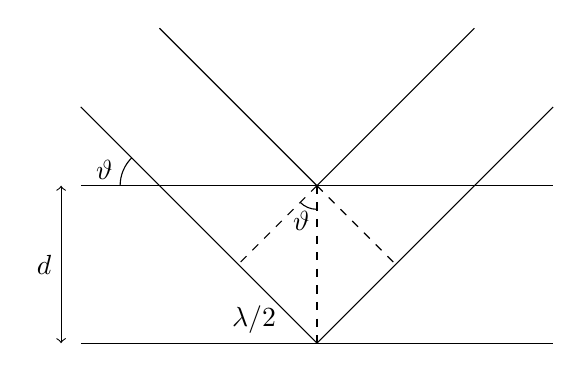
\begin{tikzpicture}
            %\draw[lightgray] (0, 0) grid (6, 4);
            \draw (0, 0) -- (6, 0);
            \draw (0, 2) -- (6, 2);
            \draw (1, 4) -- (3, 2) -- (5, 4);
            \draw (0, 3) -- (3, 0) -- (6, 3);
            \begin{scope}
                \clip (1, 2) -- (0, 2) -- (0, 3) -- cycle;
                \draw (1, 2) circle[radius=0.5];
            \end{scope}
            \node at (0.3, 2.2) {\(\vartheta\)};
            \draw[<->] (-0.25, 0) -- (-0.25, 2);
            \node[left] at (-0.25, 1) {\(d\)};
            \draw[dashed] (3, 2) -- (3, 0);
            \draw[dashed] (3, 2) -- (2, 1);
            \draw[dashed] (3, 2) -- (4, 1);
            \begin{scope}
                \clip (3, 2) -- (2, 1) -- (3, 0) -- cycle;
                \draw (3, 2) circle[radius=0.3];
            \end{scope}
            \node at (2.8, 1.55) {\(\vartheta\)};
            \node at (2.2, 0.3) {\(\lambda/2\)};
        \end{tikzpicture}
        \caption{X--ray diffraction with constructive interference}
        \label{fig:x-ray diffraction}
    \end{figure}
    It can be seen from figure \ref{fig:x-ray diffraction} that the light is in phase when
    \[\sin\vartheta = \frac{n(\lambda/2)}{d}\]
    where \(n\) is a positive integer.
    Rearranging this gives Bragg's law:
    \begin{equation}\label{eqn:Bragg's law}
        n\lambda = 2d\sin\vartheta
    \end{equation}
    This is the condition for in phase scattering from planes a distance \(d\) apart.
    This depends only on \(d\) and \(\lambda\) not on which atoms or where in the plane they are.
    
    We can use the Miller indices, \((hkl)\), of the planes to label the diffraction maxima.
    In general monochromatic light will not be reflected and either \(\lambda\) or \(\vartheta\) must be changed until Bragg's law is satisfied.
    Usually it is easier to change \(\vartheta\).
    A given lattice will have a set diffraction pattern.
    If we know \(\lambda\) and the diffraction angles then the unit cell dimensions can be deduced.
    Combining Bragg's law (equation \ref{eqn:Bragg's law}) and the equation for \(d(hkl)\) (equation \ref{eqn:d(hkl)}) for a cubic lattice we get
    \[\sin^2\vartheta = \frac{\lambda^2}{4a^2}(h^2 + k^2 + l^2)\]
    assuming first order diffraction so \(n = 1\).
    Plotting \(\sin^2\vartheta\) against \(h^2 + k^2 + l^2\) will give a straight line of gradient \(\lambda^2/4a^2\) for any cubic system.
    We will see later how the crystal structure also defines the intensities of the different orders.
    
    \section{Diffraction Orders}
    \subsection{Higher Order Diffraction}
    In Bragg's law (equation \ref{eqn:Bragg's law}) the factor of \(n\) determines the order of diffraction.
    Consider a cubic crystal with lattice parameter \(a\).
    It is clear from Bragg's law that the lowest diffraction angle corresponds to the largest plane spacing and smallest value of \(n\).
    This implies that only one of \(h\), \(k\) and \(l\) is non--zero and equal to 1 and the other two are zero.
    This gives \(d = a\).
    This occurs for the \(\{100\}\) family of planes.
    The second order diffraction from \((100)\) occurs at
    \[\vartheta = \arcsin\left(2\frac{\lambda}{2a}\right) = \arcsin\left(\frac{\lambda}{a}\right)\]
    Now if we consider the \((200)\) planes we get \(d(200) = a/2= d(100)/2\).
    The angle for first order diffraction from the \((200)\) planes is
    \[\vartheta = \arcsin\left(1\frac{\lambda}{2(a/2)}\right) = \arcsin\left(\frac{\lambda}{a}\right)\]
    These angles are identical and hence the different maxima from the different planes coincide.
    For most purposes though  we only need to consider the first order diffraction as at higher orders they are much weaker.
    
    \subsection{Reflection Intensity}
    As previously mentioned the reflection intensity can be used to determine the position of atoms in the unit cell.
    Consider the body centred cubic crystal \ce{CsCl}.
    \(a = \SI{4.11}{\angstrom}\) and \(\lambda = \SI{1.54}{\angstrom}\).
    Assume
    \begin{itemize}
        \item Negligible amount of incident beam is scattered
        \item All atoms have the same amplitude of incident light
        \item Atomic reflecting power is proportional to the number of ions so \(Z - n\) for \ce{Z^{n+}} ions and \(Z + n\) for \ce{Z^{n-}} ions
    \end{itemize}
    \ce{Cs+} has \(Z = 55\) so has 54 electrons.
    \ce{Cl-} has \(Z = 17\) so has 18 electrons.
    
    First we will consider the reflection from the \((100)\) planes.
    The density of ions in each plane is identical (1 ion per \(a^2/2\) area).
    All of the \ce{Cs+} ions scatter in phase at \(\vartheta(100)\) so there is a reflection at this angle.
    However, all of the \ce{Cl-} atoms in the planes between the \(100\) planes also scatter in phase with each other at \(\vartheta(100)\) but since they are directly between the \ce{Cs+} planes this reflection is exactly out of phase so the amplitude, \(A\), of the total reflected beam from the \((100)\) planes is
    \[A(100) = (54 - 18)\cdot\text{const}\]
    where \(\text{const}\) is some constant of proportionality.
    The intensity \(I = A^2\) so
    \[I(100) = 1296\cdot\text{const}^2\]
    
    Next we consider the scattering from the \((200)\) planes.
    Now there is no plane between planes so all scattering at angle \(\vartheta(200)\) is in phase so
    \[A(200) = (54 + 18)\cdot\text{const}\]
    \[I(200) = 5184\cdot\text{const}^2\]
    The same occurs for the \((110)\) planes so they also have 
    \[I(110) = 5184\cdot\text{const}^2\]
    
    The \((111)\) planes again have a plane of \ce{Cl-} ions between them so scatter out of phase with
    \[I(111) = 1296\cdot\text{const}^2\]
    
    This analysis works well and reproduces the positions exactly and roughly the correct amplitude, it can be improved by noting that \(\text{const}\) is not the same for all reflections.
    
    \subsection{Systematic Absences}
    Considering a bcc crystal with identical atoms at the centre instead we get that when there is destructive interference since both atoms have the same number of electrons the intensities are now reduced to zero.
    These are called systematic absences.
    There are some simple conditions that determine whether a crystal of a certain structure will have a systematic absence for a particular plane.
    For first order reflection the restrictions on the possible values of \(h\), \(k\) and \(l\) for there to be no systematic intensity are
    \begin{itemize}
        \item Simple cubic: No restriction on \(h\), \(k\) or \(l\)
        \item Body centred cubic: \(h + k + l = \text{even}\) for non--zero intensity
        \item Face centred cubic: \(h\), \(k\) and \(l\) all even or all odd for non--zero intensity
    \end{itemize}
    
    \subsection{Experimental Methods of X--ray Diffraction}
    Note that if an angle is measured relative to the path the x--ray would have taken if not for the crystal (as it almost always is) then the angle measured is \(2\vartheta\).
    A detector of some sort is placed behind the crystal.
    Commonly a CCD is used now but in the past film or even and image plate would have been used.
    
    \subsubsection{Rotation Method}
    A single crystal is exposed to collimated, monochromatic x--rays.
    Initially no diffraction is expected as it is unlikely that Bragg's law will be satisfied.
    The crystal is rotated about a fixed axis perpendicular to the beam of x--rays until diffraction occurs.
    This is done to find as many diffraction angles as needed.
    
    \subsubsection{Powder Method}
    A powder of the crystal is placed in a collimated, monochromatic beam of x--rays.
    Since the powder contains crystals of all orientations diffraction will occur and causes a set of rings to appear.
    Integrating the intensity around the rings gives the total intensity.
    This method guarantees that all possible diffraction angles are found (although the intensity may be too low to actually use).
    
    \subsubsection{Laue Method}
    White (continuous spectrum) x--rays are used with a single stationary crystal.
    Each set of planes will satisfy Bragg's law for some wavelength and the resulting diffracted beams generate a pattern.
    The symmetry of the diffraction pattern reflects the symmetry of the crystal when viewed along the x--ray beam.
    
    \subsection{Types of Diffraction}
    \subsubsection{X--ray Diffraction}
    So far we have only considered x--ray diffraction
    X--rays scatter from electrons in the atom and the reflecting power of the atom depends on the number of electrons.
    Traditional x--ray tubes use a \ce{Cu} or \ce{Mo} target to produce x--rays and can produce x--rays of wavelength \(\SI{1.54}{\angstrom}\) or \(\SI{0.71}{\angstrom}\) respectively.
    X--rays can also be obtained from magnetically accelerated electron beams but this requires a lot of equipment (as in a literal particle accelerator).
    
    \subsubsection{Neutron Diffraction}
    We can obtain neutrons with a wavelength \(\sim\SI{1}{\angstrom}\).
    For this we need a neutron with a velocity \(\sim\SI{4}{km.s^{-1}}\).
    This is easily produced by a fission reaction.
    The neutrons scatter off of the nucleus of the atoms.
    The reflection power does not vary simply with atomic number.
    It depends heavily on the properties of the nucleus.
    
    \section{Vibrating Solids}
    \subsection{Harmonic Oscillators}\label{sec:harmonic oscillators}
    Vibrations of bonded atoms are important whenever there is a bond in a single molecule or a large crystal.
    Two particles are joined by a bond with a potential given by the Lennard--Jones potential:
    \[U(r) = 4\epsilon\left[\left(\frac{\sigma}{r}\right)^{12} - \left(\frac{\sigma}{r}\right)^6\right]\]
    The equilibrium separation is \(r_0 = 2^{1/6}\sigma \approx 1.12\sigma\) which corresponds to the deepest part of the potential well where \(U(r_0) = -\varepsilon\).
    
    In reality particles don't just sit at the equilibrium separation.
    They oscillate around it.
    Classically any system with non--zero thermal energy must have some vibrational energy.
    In the quantum view vibrations have some non--zero zero point energy.
    The potential is almost symmetric near the base of the potential well and as such oscillations of a small amplitude are approximately harmonic.
    To see this we Taylor expand the Lennard--Jones potential:
    \[U(r) = U(r_0) + U'(r_0)(r - r_0) + \frac{U''(r_0)}{2!}(r - r_0)^2 + \frac{U'''(r_0)}{3!}(r - r_0)^3 + \mathcal{O}\left((r - r_0)^4\right)\]
    \[U(r_0) = -\epsilon,\qquad U'(r_0) = 0,\qquad U''(r_0) = \frac{4\epsilon}{\sigma}\frac{18}{2^{1/3}},\qquad U'''(r_0) = -\frac{4\epsilon}{\sigma}\frac{378}{2^{1/2}}\]
    \[U(r) = -\epsilon\left[1 - \frac{2^{2/3}\cdot 18}{\sigma^2}(r - r_0)^2 + \frac{2^{1/2}\cdot 126}{\sigma^3}(r - r_0)^3 + \mathcal{O}\left((r - r_0)^4\right)\right]\]
    Considering only small displacements and so disregarding higher order terms we get
    \[U(r)\approx -\epsilon + \epsilon\frac{2^{2/3}\cdot 18}{\sigma^2}(r - r_0)^2\]
    This second order expansion has the same form as a simple harmonic oscillator of potential \(u(x)\):
    \[u(x) = u_0 + \frac{1}{2}k_\text{spring}x^2\]
    Where \(k_\text{spring}\) is the ``spring constant" and is
    \[k_\text{spring} = (2^{2/3}\cdot 36)\frac{\epsilon}{\sigma^2}\]
    This turns out to be a fairly good approximation.
    The particle will oscillate at angular frequency
    \[\omega = \sqrt{\frac{k_\text{spring}}{m}}\]
    where \(m\) is the mass of the particle.
    For the Lennard--Jones potential we get
    \[\omega = \frac{2^{1/3}\cdot 6}{\sigma}\sqrt{\frac{\epsilon}{m}}\]
    For argon with \(m = \SI{40}{amu}\) this gives \(\omega = \SI{3.45e12}{rad.s^{-1}}\) so the atom oscillates at \(f = \omega/2\pi = \SI{5.5e11}{s^{-1}} = \SI{0.55}{\tera Hz}\) and has period \(T = 1/f = \SI{1.8e-12}{s} = \SI{1.8}{\pico s}\).
    This is actually relatively slow compared to other materials with stronger bonding, note that \(f\) scales as \(\sqrt{\epsilon}\).
    
    \subsection{Heat Capacity of Solids}
    Bonds in the solid state can execute nearly harmonic motion in the form of vibrations.
    These vibrations carry thermal energy and as such will contribute to its heat capacity.
    Recall that for an ideal gas at constant volume:
    \begin{itemize}
        \item Monatomic gases have 3 degrees of freedom from translations in three directions so have a heat capacity of
        \[C_V = 3\cdot\frac{1}{2}R = \frac{3}{2}R\]
        \item Diatomic gases have, in addition to the translational degrees of freedom:
        \begin{itemize}
            \item 2 rotational degrees of freedom for orthogonal rotations to the bond axis. Each contributes
            \[2\cdot\frac{1}{2}R = R\]
            for a total heat capacity of
            \[C_V = \frac{3}{2}R + R = \frac{5}{2}R\]
            \item 1 vibrational degree of freedom with a potential and kinetic quadratic mode contributing
            \[2\cdot\frac{1}{2}R =R\]
            for a total heat capacity of
            \[C_V = \frac{3}{2} + R + R = \frac{7}{2}R\]
        \end{itemize}
        \item The temperature must be sufficiently high for these degrees of freedom to be accessible.
    \end{itemize}
    This is all for a gas, but what about a solid?
    In a solid the particles aren't free to move about, instead they are confined by their position in the lattice, this is like being enclosed in a small box.
    Hence translational degrees of freedom are not available.
    Bonds between particles in the crystal can't rotate so rotational degrees of freedom aren't free.
    Particles can vibrate and as such only vibrational modes are available.
    Vibration can occur in any three orthogonal directions and each direction has a kinetic and potential quadratic mode.
    
    \subsection{Classical Picture of Solid Heat Capacity}
    Consider a simple cubic crystal.
    Each atom is bonded to its 6 nearest neighbours.
    Each bond can be approximated as a harmonic potential.
    We can model this as each particle being suspended by 6 springs running along the positive and negative coordinate axes.
    For now we will ignore the fact that the vibrational modes are quantised and assume we are at a high enough temperature that they are all available.
    For each particle in the lattice there are three independent harmonic oscillators in the \(x\), \(y\) and \(z\) directions having energy similar to
    \[u_x = \frac{1}{2}k(x - x_0)^2 + \frac{1}{2}mv_x^2\]
    And an average energy given by
    \[\expval{u_x} = \frac{1}{2}k\expval{(x - x_0)^2} + \frac{1}{2}m\expval{v_x^2}\]
    Each degree of freedom then contributes \(0.5R\) to the heat capacity so the heat capacity is
    \[C_V = 6\cdot\frac{1}{2}R = 3R = \SI{24.94}{J.mol^{-1}.K^{-1}}\]
    This was first observed experimentally by Dulong and Petit and is referred to as the law of Dulong and Petit.
    However it isn't the complete picture.
    It works well when bonds aren't too strong which can be seen in table and only near room temperature.
    \ref{tab:dulong petit}
    \begin{table}[ht]
        \centering
        \begin{tabular}{c|c}\hline
            Material & \(C_V/R\)\\\hline
            Copper & 2.92\\
            Aluminium & 2.82\\
            Gold & 3.03\\
            Lead & 3.21\\
            Iron & 2.98\\
            Sodium & 3.32\\
            \ce{NaCl} & 2.96\\
            Silicon & 2.62\\
            Diamond & 0.60
        \end{tabular}
        \caption{The value of \(C_V/R\) for some common materials at \SI{300}{K}}
        \label{tab:dulong petit}
    \end{table}
    This rule is also known as the Dulong Petit limit as \(C_V = 3R\) is the limiting value reached at high temperatures.
    This is due to the quantum nature of the vibrational degrees of freedom and the fact that stronger bonds have higher values of \(k\) and therefore are further apart so not available until a higher temperature is reached.
    
    \subsection{Quantum Picture of Solid Heat Capacity}
    Like molecular vibrations lattice vibrational energies are quantised.
    The difference between energy levels is comparable to thermal energies.
    We start with a quantum harmonic oscillator with energy
    \[\epsilon_n = \left(n + \frac{1}{2}\right)\hbar\omega\]
    where \(n = 0, 1, 2,\dotsc\)
    The energy needed to excite the system from its ground state (\(n = 0\), \(\epsilon_0 = 0.5\hbar\omega\)) is \(\hbar\omega\).
    Hence thermal energies must be of a similar order so \(k_BT\sim\hbar\omega\) to allow for excitation into higher vibrational states.
    Recall in section \ref{sec:harmonic oscillators} the angular frequency for argon was found to be \(\omega = \SI{3.45e12}{rad.s^{-1}}\) so the temperature at which a significant population of excited vibrational modes is possible is
    \[T\sim \frac{\hbar\omega}{k_B} = \SI{165}{K}\]
    Below this temperature excited vibrational modes are mostly unavailable.
    The boiling point of argon at atmospheric pressure is \SI{83}{K} so argon doesn't normally reach this Dulong Petit limit unless the pressure is much greater than atmospheric pressure.
    
    At sufficiently low temperatures we expect that no vibrational degrees of freedom are available and as such the heat capacity drops to zero.
    This same behaviour does not occur for an ideal gas which always has translational degrees of freedom since these are classical and always available.
    
    \subsection{Einstein Model}
    A simple and empirically successful model to track the occupation of excited vibrational modes is the Einstein Model.
    Consider the energy of a simple harmonic oscillator in one dimension:
    \[\epsilon_n = \left(n + \frac{1}{2}\right)\hbar\omega\]
    We redefine energy levels as the energy above the zero point energy of \(0.5\hbar\omega\) so
    \[\epsilon_n = n\hbar\omega\]
    we will add the zero point energy back in later.
    We can use the Boltzmann factor to describe the spread over the different states at a specific temperature:
    \[N_n = A\exp\left(-\frac{\epsilon_n}{k_BT}\right) = A\exp\left(-\frac{n\hbar\omega}{T}\right) = A\exp(-n\chi)\]
    where \(\chi = \hbar\omega/k_BT\).
    To determine the value of the constant \(A\) we require that the total number of states across all atoms is equal to the number of oscillators, \(N\):
    \[N = \sum_{n = 0}^\infty N_n = \sum_{n = 0}^\infty Ae^{-n\chi}\]
    Some useful exponential series rules here are
    \[\sum_{n = 1}^\infty e^{-kz} = \frac{1}{e^z - 1},\qquad \sum_{n = 0}^0 e^{-kz} = e^0 = 1\]
    \[N = \sum_{n = 0}^\infty Ae^{-n\chi} = \sum_{n = 1}^\infty Ae^{-n\chi} + \sum_{n = 0}^0 Ae^{-n\chi}\]
    \[= \frac{1}{e^{\chi} - 1} + 1 = \frac{1}{e^{\chi} - 1} + \frac{e^{\chi} - 1}{e^{\chi} - 1} = \frac{1 + e^{\chi} - 1}{e^{\chi} - 1} = \frac{e^{\chi}}{e^{\chi} - 1} = \frac{1}{1 - e^{-\chi}}\]
    Rearranging we get
    \[A = N(1 - e^{-\chi})\]
    So the number of atoms in the \(n^\text{th}\) state is
    \[N_n = N(1 - e^{-\chi})e^{-n\chi}\]
    The total energy for vibrations summed over all particles is
    \[U = \sum_{n = 0}^\infty N_n\epsilon_n = \sum_{n = 1}^\infty\left[N(1 - e^{-\chi})e^{-n\chi}n\hbar\omega\right]\]
    Note that the sum starts as \(n = 0\) but after substitution is from \(n = 1\).
    This is allowed as \(\epsilon_0 = 0\) since we took this as the base energy for all others.
    Considering a molar amount and that there are three independent dimensions we get \(N = 3N_A\) and
    \[U = 3N_A\sum_{n = 1}^\infty \left[n\hbar\omega(1 - e^{-\chi})e^{-n\chi}\right]\]
    This sum can be simplified:
    \begin{align*}
        U &= 3N_A\sum_{n = 1}^\infty \left[n\hbar\omega(1 - e^{-\chi})e^{-n\chi}\right]\\
        &= 3N_A\hbar\omega\sum_{n = 1}^\infty\left[ne^{-n\chi} - ne^{-\chi}e^{-n\chi}\right]\\
        &= 3N_A\hbar\omega\sum_{n = 1}^\infty\left[ne^{-n\chi} - ne^{-(n + 1)\chi}\right]\\
        &= 3N_A\hbar\omega\sum_{n = 1}^\infty\left[ne^{-n\chi} - ne^{-(n + 1)\chi} - e^{-(n + 1)\chi} + e^{-(n + 1)\chi}\right]\\
        &= 3N_A\hbar\omega\sum_{n = 1}^\infty\left[ne^{-n\chi} - (n + 1)e^{-(n + 1)\chi} + e^{-(n + 1)\chi}\right]\\
        &= 3N_A\hbar\omega\left[\sum_{n = 1}^\infty ne^{-n\chi} - \sum_{n = 2}^\infty ne^{-n\chi} + \sum_{n = 2}^\infty e^{-n\chi}\right]\\
        &= 3N_A\hbar\omega\left[e^{-\chi} + \sum_{n = 2}^\infty ne^{-n\chi} - \sum_{n = 2}^\infty ne^{-n\chi} + \sum_{n = 2}^\infty e^{-n\chi}\right]\\
        &= 3N_A\hbar\omega\left[e^{-\chi} + \sum_{n = 2}^\infty e^{-n\chi}\right]\\
        &= 3N_A\hbar\omega\sum_{n = 1}^\infty e^{-n\chi}
    \end{align*}
    Which using the rules for sums of exponentials from before is
    \[U = \frac{3N_A\hbar\omega}{e^{\chi} - 1} = \frac{3N_A\hbar\omega}{\exp(\hbar\omega/k_BT) - 1}\]
    Finally we add the zero point energy back as a constant shift for all of the \(3N_A\) nodes:
    \[U = 3N_A\hbar\omega\left[\frac{1}{2} + \frac{1}{\exp(\hbar\omega/k_BT) - 1}\right]\]
    The heat capacity at constant volume is
    \begin{align*}
        C_V &= \pdvconst{U}{T}{V}\\
        &= \frac{\hbar\omega\exp(\hbar\omega/k_BT)}{k_BT^2} \frac{3N_A\hbar\omega}{[\exp(\hbar\omega/k_BT) - 1]^2}\\
        &= 3N_Ak_B\left(\frac{\hbar\omega}{k_BT}\right)^2 \frac{\exp(\hbar\omega/k_BT)}{[\exp(\hbar\omega/k_BT) - 1]^2}\\
        &= 3R\left(\frac{\vartheta_E}{T}\right)^2\frac{\exp(\vartheta_E/T)}{[\exp(\vartheta_E/T) - 1]^2}
    \end{align*}
    Where we have used the fact that \(N_Ak_B = R\) and defined the Einstein temperature \(\vartheta_E = \hbar\omega/k_B\).
    This is the Einstein Model for specific heat.
    This form of the Einstein temperature is the same as the order of magnitude estimate for the temperature at which excited states are populated in a quantum harmonic oscillator.
    
    At high temperatures
    \[\exp\left(\frac{\hbar\omega}{k_BT}\right) \approx 1 + \frac{\hbar\omega}{k_BT} = 1 + \frac{\vartheta_E}{T}\]
    so the Einstein model reduces to
    \[C_V \approx 3R\left(\frac{\vartheta_E}{T}\right)^2\frac{1 + \vartheta_E/T}{(\vartheta_E/T)^2} = 3R\left(1 + \frac{\vartheta_E}{T}\right)\]
    \[C_V \approx 3R\]
    assuming that the \(\vartheta_E/T\) term is negligible.
    This agrees with the earlier analysis that lead to the Dulong Petit law.
    The Einstein model works well at high temperatures but at low temperatures requires a fix given in the Debye model for heat capacity.
    
    \section{Debye Model for Heat Capacity}
    So far we have assumed that the lattice is fixed apart from one molecule which is oscillating.
    In reality all molecules are oscillating and we need to consider these coupled oscillations to get a full picture.
    We consider phonons which are the wave-like collective vibrations of the whole lattice.
    In the Debye model the phonons are treated as standing waves or normal modes of the lattice but it is possible to treat them as a particle as well.
    The Debye phonons have a range of frequencies.
    The lower the frequency the longer the length scale over which the phonon needs to be considered.
    The Einstein Model can be thought of as only dealing with high frequency phonons and hence only close by oscillation.
    As temperature is lowered the high frequency modes become unavailable so the low frequency modes are more populated which is why the Einstein model fails at low temperatures.
    
    By considering lower frequency modes the Debye model makes a higher prediction for lower temperatures than the Einstein model does.
    The Debye model is
    \[C_V = 9R\left(\frac{T}{\vartheta_D}\right)^3 \int_0^{\vartheta_D/T}\frac{x^4e^x}{(e^x - 1)^2}\,\dd x\]
    where \(\vartheta_D\) is the Debye frequency.
    The integral does not have a closed form solution.
    \(\vartheta_D\) is analogous to \(\vartheta_E\) and indeed, they usually have similar values.
    We can also define the Debye frequency \(\omega_D = k_B\vartheta_D/\hbar\).
    This represents the maximum phonon frequency of the lattice.
    
    The Debye model is so accurate that \(\vartheta_D\) is considered a fundamental material constant.
    Because it characterises the vibrational properties of the material it is useful for more than just specifying heat capacities.
    For example it can be seen that the higher the value of \(\vartheta_D\) (or \(\vartheta_E\)) the stronger the bonds are.
    For example for lead \(\vartheta_D = \SI{88}{K}\) and for diamond \(\vartheta_D = \SI{1860}{K}\).
    This corresponds to the fact that lead is much softer than diamond.
    
    Even the Debye model still makes assumptions about the behaviour of phonons.
    In the Einstein model it is assumed that all phonons are oscillating at  frequency \(\omega\).
    The Debye model assumes that all phonons are oscillating at less than \(\omega_D\) and are distributed with more at higher temperature increasing smoothly.
    The more advanced density functional theory uses the density of states to give a more accurate prediction based on which states are filled.
    For most cases the Debye model is more than good enough.
    
    \subsection{Solid Heat Capacity at constant Pressure}
    So far we have only dealt with heat capacity at a constant volume for solids and like gases the heat capacity at a constant pressure is different.
    In practice  the heat capacity at constant pressure is best determined empirically.
    It is often assumed for solids that \(C_p\) and \(C_V\) are approximately the same.
    The heat capacity at constant volume \emph{and} pressure is
    \[C_{V,p} = \pdvconst{Q}{T}{V,p}\]
    \[\dd U = \dd Q + \dd W\]
    \[\dd Q = \dd U + p\dd V\]
    Internal energy, \(U\), is usually specified by the thermodynamic variables \(T\) and \(V\).
    \[U = U(T, V)\]
    \[\dd U = \pdvconst{U}{T}{V}\dd T + \pdvconst{U}{V}{T}\dd V\]
    \[\dd Q = \pdvconst{U}{T}{V}\dd T + \left[\pdvconst{U}{V}{T} + p\right]\dd V\]
    \[C_p = \pdvconst{U}{T}{V} + \left[\pdvconst{U}{V}{T} + p\right]\pdvconst{V}{T}{p}\]
    \[C_V = \pdvconst{U}{T}{V}\]
    \[C_p - C_V = \left[\pdvconst{U}{V}{T} + p\right]\pdvconst{V}{T}{p}\]
    For an ideal gas the internal energy only depends on  temperature so we only keep the \(p\) as the internal energy is constant with volume so the first term is zero.
    \[U = f(t)\]
    \[C_p - C_V = p\pdvconst{V}{T}{p}\]
    \[V = \frac{RT}{p}\]
    \[C_p - C_V = R\]
    For an ideal, monatomic, gas \(C_V = 3R/2\) so
    \[\frac{C_p - C_V}{C_V} = \frac{R}{3R/2} = \frac{2}{3} = \SI{67}{\%}\]
    so the difference between \(C_p\) and \(C_V\) is significant.
    For a solid the internal energy depends on temperature and volume so we have to keep both terms.
    \[U = f(T, V)\]
    \[C_p - C_V = \left[\pdvconst{U}{V}{T} + p\right]\pdvconst{V}{T}{p}\]
    At finite temperatures \((\partial V/\partial_T)_p\) (the thermal expansion) is very small.
    This means that \(C_p - C_V\) is very small so \(C_p\approx C_V\).
    
    The reason that \(C_P\) is higher than \(C_V\) for a gas is that the gas must do work on its surroundings to expand so it can stay at a constant pressure.
    A solid doesn't need to expand that much when heated to keep a constant pressure and so it doesn't need to do much work on its surroundings.
    
    Alternatively for a solid as \(T\to 0\) \(C_V\to 0\).
    \[\dd U = T\dd S - p\dd V = -p\dd V\]
    \[\pdvconst{U}{V}{T} = -p\]
    \[C_p - C_V = \left[\pdvconst{U}{V}{T} + p\right]\pdvconst{V}{T}{p} = \left[-p + p\right]\pdvconst{V}{T}{p} = 0\]
    The fact that \(C_V\to 0\) as \(T\to 0\) is a separate, quantum phenomenon.
    
    \subsection{Thermal Expansion of Solids}
    Solids expand as they are heated however in our harmonic approximation while at high temperatures the maximum deviation from the equilibrium position may increase the average position is still the same.
    How does a solid expand with \(T\) if the average bond length doesn't change?
    The answer is that the interatomic potential is not actually symmetrical as assumed for the harmonic approximation.
    This means that oscillations aren't entirely harmonic.
    The Taylor series of the Lennard--Jones potential is
    \[U(r) = -\epsilon\left[1 - \frac{2^{2/3}\cdot 18}{\sigma^2}(r - r_0)^2 + \frac{2^{1/2}\cdot 126}{\sigma^3}(r - r_0)^3 + \mathcal{O}\left((r - r_0)^4\right)\right]\]
    Before we truncated at the \((r - r_0)^2\) term.
    If we keep the next term we better reproduce the asymmetry of the potential.
    This additional term beyond the harmonic term is called the anharmonic term and is proportional to \((r - r_0)^3\).
    As the vibrational energy increases the mean position of the vibrating bond length will shift to positive \(r\) with temperature, away from the ``cold" equilibrium position, \(r_0\).
    So the anharmonic nature of the true potential is the reason for thermal expansion.
    However since the anharmonic terms are so small the bond length doesn't change by that much so the thermal expansion is small.
    The thermal expansivity, \(\beta\), is
    \[\beta = \frac{1}{V}\pdvconst{V}{T}{p}\]
    For an ideal gas
    \[V = \frac{RT}{p}\implies \frac{1}{V} = \frac{p}{RT}\]
    \[\pdvconst{V}{T}{p} = \frac{R}{p}\implies \beta_\text{gas} =  \frac{p}{RT}\frac{R}{p} = \frac{1}{T}\]
    \[\beta_\text{gas} = \frac{1}{T} \approx \SIrange[range-phrase=-]{e-2}{e-3}{K^{-1}}\]
    near ambient conditions.
    For solids
    \[\beta_\text{solid} \approx \SIrange[range-phrase=-]{e-4}{e-5}{K^{-1}}\]
    so the thermal expansivity of solids is 10 to 1000 times smaller than for a gas.
    
    \subsection{Thermal Conductivity of Solids}
    Energy is transported across crystals by some carrier of energy such as a phonon, electron, photon, etc.
    For insulators the energy is transported by atomic motion such as vibrations, phonons and sound waves.
    In the case of metals the free electrons carry the bulk of the thermal energy.
    For now we consider the case of insulators.
    If there is a temperature difference between two regions in thermal contact then we know that they will tend toward thermal equilibrium with each other.
    In fluids mixing and flow make heat transfer a fast but complicated process following fluid dynamic as well as thermodynamic laws.
    In a solid there can't be mixing or flowing and all heat is spread only by conduction.
    This is significantly slower but much simpler.
    
    We have a steady state, one dimensional, heat transfer.
    We can write the heat flux, \(q\), which is the heat flow per unit area as
    \[q = \frac{1}{A}\dv{Q}{t}\]
    where \(A\) is the area and \(\dd Q/\dd t\) is the rate of heat flow.
    Fourier's law relates this to the gradient:
    \[q = -\kappa\dv{T}{x}\]
    where \(\kappa\) is the thermal conductivity.
    In the case of non--steady state heat transfer in one dimension the relationship is
    \[\pdv{T}{t} = D\pdv[2]{T}{x}\]
    This comes from the continuity equation, which in one dimension is
    \[\pdv{\varphi}{t} = -\pdv{q}{x}\]
    in this context \(\dd \varphi\) is the energy change per volume:
    \[\dd\varphi = \rho C_p\dd T\]
    Substituting in the expression for \(q\) from Fourier's law we get
    \[\pdv{T}{t} = \frac{\kappa}{\rho C_p}\pdv[2]{T}{x} = D\pdv[2]{T}{x}\]
    where \(D = \kappa/\rho C_p\) is the thermal diffusivity.
    Looking at the units of \(D\) we see
    \[[D] = \frac{\text{length}^2}{\text{time}}\]
    for an object of size \(\ell\) we may suppose that the cooling time is
    \[\tau \sim \frac{\ell^2}{D}\]
    
    \example
    Consider a chicken, which is mostly water \((D = \SI{e-7}{m^2.s^{-1}})\), which is \(\SI{0.2}{m}\) in diameter.
    The chicken is placed in a hot oven.
    The time taken for the chicken to reach thermal equilibrium is to an order of magnitude
    \[\tau = \frac{(\SI{0.1}{m})^2}{\SI{e-7}{m^2.s^{-1}}} = \SI{100000}{s} = \SI{28}{hrs}\]
    In reality to cook something we don't need it to reach thermal equilibrium with the oven, rather we have a desired temperature of say \SI{70}{\SIUnitSymbolDegree C} and an oven of \SI{200}{\SIUnitSymbolDegree C}.
    This only takes a few hours to happen.
    A more accurate estimate can be made by assuming a spherical chicken and solving the time dependent heat equation.
    This gives a similar amount of time, within a factor of 2 of our answer of \SI{28}{hrs}, for the time to reach thermal equilibrium.
    
    \subsection{Lattice Thermal Conductivity}
    The thermal conductivity \(\kappa\) is generally a result of three primary microscopic transport processes:
    \begin{itemize}
        \item Conduction by lattice vibrations, known as lattice conduction, has associated thermal conductivity \(\kappa_l\), this is what we covered above
        \item Conduction by free electrons, known as electronic conduction, has associated thermal conductivity \(\kappa_e\), see the section on this later
        \item Conduction by photons, known as radiative conduction, has associated thermal conductivity \(\kappa_r\), relevant mainly at high temperatures
    \end{itemize}
    The total thermal conductivity is
    \[\kappa = \kappa_l + \kappa_e + \kappa_r\]
    For an insulator near room temperature this is approximately \(\kappa - \kappa_l\).
    As an analogy to the kinetic theory of gases we can write the thermal conductivity as
    \[\kappa = \frac{1}{3}n\expval{v}\lambda C_V\]
    where \(n\) is the number density, \(v\) is the velocity of the vibration and \(\lambda\) is the mean free path of the vibration.
    
    Einstein proposed that heat could be transported by a random walk of localised (Einstein) oscillations.
    We consider the oscillations to transfer there energy every half a period as this is how long it takes to bounce between neighbours.
    This time is \(\tau_E\).
    From our previous treatment of the Einstein temperature we get
    \[\tau_E = \frac{1}{2}\frac{2\pi}{\omega} = \frac{\hbar\pi}{k_B\vartheta_E}\]
    We take \(C_V\) per atom from the Einstein model:
    \[C_V = 3k_B\frac{x^2e^x}{(e^x - 1)^2}\]
    where \(x = \vartheta_E/T\).
    The scattering length is approximately the distance between atoms which is
    \[\lambda = V^{-1/3} = n^{-1/3}\]
    Similarly the effective velocity of the atom is
    \[v = \frac{\lambda}{\tau_E} = \frac{^{-1/3}}{\tau_E}\]
    Combining this we get
    \[\kappa = \frac{k_B^2\vartheta_E}{\hbar\pi}\frac{x^2e^x}{(e^x - 1)^2}n^{1/3}\]
    This works well for amorphous solids where each atom can be thought of as an independent oscillator but for crystals we have already seen that we need to consider phonons across all length scales.
    For this reason crystals actually transmit heat faster than amorphous solids.
     
    This model can be better fitted to the empirical results for a crystal if we treat \(v\) as an elastic wave velocity in the lattice (ie the speed of sound) or as the speed of an acoustic (travelling) phonon.
    This gives a mean free path larger than the interatomic spacing which shows the need for consideration of large scale vibrations in a crystal.
    
    \section{Mechanical Properties of Solids}
    A stress is a force per unit area (like a pressure but directional).
    An elastic response to a stress is one with a reversible deformation.
    An inelastic response is not reversible.
    Fluids, by definition, have a purely inelastic response to a stress (excluding weird, non--Newtonian fluids).
    We are only going to consider mechanically isotropic solids here.
    These are solids where the mechanical properties are independent of the sample orientation.
    Crystals have intrinsic anisotropic mechanical properties but in the case of multiple small crystals such as in a crystalline solid these tend to cancel.
    
    \subsection{Elasticity}
    For an elastic deformation there is generally an applied stress, \(\sigma\), causing a resulting strain, \(\varepsilon\).\footnote{Both \(\varepsilon\), the strain, and \(\epsilon\), the binding energy, are being used in this section}
    These are proportional with the constant of proportionality, \(C\), being called the elastic modulus.
    \[\sigma = C\varepsilon\]
    \(\sigma\) is a force per unit area and has units of \(\si{N.m^{-2}}\) and \(\varepsilon\) is a fractional strain and is dimensionless.
    This means that \(C\) has units of \(\si{N.m^{-2}}\).
    We will consider several common deformations.
    
    \subsection{Compressibility: The Bulk Modulus}
    The simplest deformation occurs when the stress, \(\sigma\), is the same everywhere. 
    This is known as an isotropic stress (isotropic meaning same everywhere), hydrostatic stress (hydrostatic meaning as if the stress where from submersion in a fluid) or simply a pressure, denoted \(p\).
    For a small change, \(\Delta V\), in the volume, \(V\) the stress strain relationship is
    \[\Delta p = -K\frac{\Delta}{V}\]
    where \(K\) is a constant known as the bulk modulus.
    In differential form this is
    \[K = -V\pdv{p}{V}\]
    Taking the partial derivative under specific conditions such as constant temperature or entropy gives slightly different constants denoted \(K_T\) and \(K_S\) respectively.
    
    \(K\) is an elastic constant but it is also a thermodynamic constant and relates volume and pressure changes.
    The higher \(K\) is the less compressible a material is.
    The compressibility of a material is \(B\) and is given by
    \[B = \frac{1}{K}\]
    We can estimate \(K\)  from the lattice potential and the thermodynamic relationship:
    \[\dd U = T\dd S - p\dd V\]
    Assuming an isothermal process at \(T = \SI{0}{K}\) this is
    \[\dd U = -p\dd V\]
    \[-p = \pdvconst{U}{V}{T}\]
    Hence the bulk modulus at constant temperature is
    \[K_T = -V\pdvconst{p}{V}{T} = V\pdvconst[2]{U}{V}{T}\]
    This is then evaluated by assuming that \(r = V^{1/3}\) so \(U(r) = U(V^{1/3})\).
    
    \example
    For \ce{NaCl} we have the potential per atom of
    \[U(r) = 0.741\epsilon\left[6\left(\frac{\sigma}{r}\right)^9 - 1.75\left(\frac{\sigma}{r}\right)\right]\]
    Hence the potential in terms of volume is
    \[U = 0.741\epsilon\left[6\sigma^9V^{-3} - 1.75\sigma V^{-1/3}\right]\]
    \[\pdvconst{U}{V}{T} = 0.741\epsilon\left[6(-3)\sigma^9V^{-4} - 1.75\left(-\frac{1}{3}\right)\sigma V^{-4/3}\right]\]
    \begin{align*}
        \pdvconst[2]{U}{V}{T} &= 0.741\epsilon\left[6(-3)(-4)\sigma^9 V^{-5} - 1.75\left(-\frac{1}{3}\right)\left(-\frac{4}{3}\right)\sigma V^{-7/3}\right]\\
        &= 0.741\epsilon\left[72\sigma^9 V^{-5} - 0.778\sigma V^{-7/3}\right]
    \end{align*}
    \[K_T = V\pdvconst[2]{U}{V}{T} = 0.741\epsilon\left[72\sigma^9 V^{-4} - 0.778\sigma V^{-4/3}\right]\]
    This gives \(K_T\) as a function of the ionic volume.
    To find \(K_T\) at the equilibrium volume insert the equilibrium value \(V = r_1^3\) where \(r_1 = 1.54\sigma\) and \(\sigma = \SI{1.83}{\angstrom}\).
    \begin{align*}
        K_T &= 0.741\epsilon\left[72\left(\frac{r_1}{1.54}\right)^9\left(r_1\right)^{-4} - 0.778\left(\frac{r_1}{1.54}\right)\left(r_1^3\right)^{-4/3}\right]\\
        &= 0.741\epsilon[1.47 - 0.505]r_1^{-3}\\
        &= 0.2\frac{\epsilon}{\sigma^3}\\
        &= \SI{21e9}{Pa} = \SI{21}{\giga Pa}
    \end{align*}
    This is close to the experimental value of \SI{23.8}{\giga Pa}.
    Elastic moduli are typically measured in \si{\giga Pa}.
    
    According to our model changing the volume of the crystal by applying a stress or changing the temperature will effect the elastic constants of the material.
    
    The bulk modulus increases with compression.
    In terms of the interatomic potential this is because the repulsive force increases as atoms are forced closer together so it becomes harder to compress the material so the bulk modulus must increase.
    Integrating the stress strain relationship we ge that to make a certain compression we need a pressure given by
    \[p = \int\dd p = -\int\frac{K}{V}\,\dd V\]
    If the volume change is small then we use the linear elastic approximation where \(K_T\) is a constant so
    \[\Delta p = -K_T\frac{\Delta V}{V}\]
    
    The bulk modulus decreases with expansion as the distance between atoms decreases so the effects of the repulsive term decrease.
    This effect is called softening.
    Since increasing temperature causes an expansion the effect of increasing temperature is to soften a material.
    The limit of this is when the material becomes a liquid or even a gas when it becomes very compressible compared to a solid.
    
    \subsection{Young's Modulus}
    If a force \(F\) is applied in one direction to a material with cross sectional area \(A\) perpendicular to the force then we call this a uniaxial stress.
    The force causes the material to extend from a length \(x\) by a small amount \(\Delta x\).
    Equally it could cause a compression by the same amount and the same maths would hold.
    The stress strain behaviour is given by Young's modulus, \(E\).
    For a small deformation
    \[\frac{F}{A} = E\frac{\Delta x}{x}\]
    Consider an atomic bond parallel to the force.
    If the bond length before the force is applied is \(r_0\) and it is stretched by \(x\) by the force then we can use the harmonic approximation of the potential to describe the deformation:
    \[U(x) = U_0 + \frac{1}{2}k(x)^2\]
    where for the Lennard--Jones potential the spring constant is
    \[k = \frac{\epsilon(2^{2/3}\cdot 36)}{\sigma^2} = \frac{72\epsilon}{r_0^2}\]
    The force applied to a spring is equal and opposite to the restoring force so
    \[F = -\left(-\dv{U}{x}\right) = kx\]
    The force is applied over an area \(A = r_0^2\) assuming a cubic lattice.
    Hence
    \[\sigma = \frac{F}{A} = \frac{kx}{r_0^2}\]
    The strain is
    \[\varepsilon = \frac{x}{r_0}\]
    so the Young's modulus is
    \[E = \frac{\sigma}{\varepsilon} = \frac{72\epsilon}{r_0^2}\frac{x}{r_0^2}\frac{r_0}{x} = \frac{72\epsilon}{r_0^3}\]
    For argon this gives a value of \(E\approx\SI{2}{\giga Pa}\) which compares favourably with experimental values of \(E = \SIrange[range-phrase=-]{2}{3}{\giga Pa}\).
    If instead we assume a fcc structure then we find that
    \[E = \frac{77\epsilon}{r_0^3}\]
    which is slightly better.
    
    \subsection{Shear Modulus}
    A stress applied parallel to a surface is called a shear stress.
    A shear deformation is characterised by the shear modulus, \(\mu\).
    \begin{figure}[ht]
        \centering
        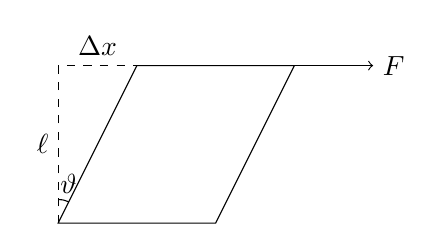
\begin{tikzpicture}
            \draw (0, 0) -- (2, 0) -- (3, 2) -- (1, 2) -- cycle;
            \draw[dashed] (0, 0) -- (0, 2) -- (1, 2);
            \node[above] at (0.5, 2) {\(\Delta x\)};
            \node[left] at (0, 1) {\(\ell\)};
            \begin{scope}
                \clip (0, 0) -- (0, 2) -- (1, 2) -- cycle;
                \draw (0, 0) circle[radius=0.3];
            \end{scope}
            \node at (0.13, 0.5) {\(\vartheta\)};
            \draw[->] (3, 2) -- (4, 2);
            \node[right] at (4, 2) {\(F\)};
        \end{tikzpicture}
        \caption{Shear stress}
        \label{fig:shear stress}
    \end{figure}
    Consider the deformation shown in figure \ref{fig:shear stress}.
    If the area of the face parallel to the force is \(A\) then
    \[\frac{F}{A} = \mu\frac{\Delta x}{\ell} \approx \mu\vartheta\]
    using the small angle approximation.
    
    \subsection{Poisson's Ratio}
    Going back to uniaxial stress (as with Young's modulus).
    If the bar is stretched then there must be contraction in the perpendicular directions.
    This is characterised by Poisson's ration, \(\nu\).
    Poisson's ratio is the strain perpendicular to the stress divided by the strain parallel to the stress.
    In the 2D case a stress in the \(y\) direction causes a longitudinal strain \(\varepsilon_L = y/\Delta y\) where \(\Delta y\) is the expansion in the \(y\) direction from initial length \(y\).
    A the same time the stress also causes a translational stress \(\varepsilon_T = \Delta x/x\) where \(\Delta x\) is the contraction along the \(x\) direction from the original length \(x\).
    This gives a Poisson's modulus of
    \[\nu = \frac{\varepsilon_T}{\varepsilon_L} = \frac{\Delta x/x}{\Delta y/y} = \frac{y\Delta x}{x\Delta y}\]
    In reality things aren't 2D.
    A cube, side length \(L\), with a stress applied perpendicular to one face extends by a length \(\Delta L\) along the direction of the stress.
    The other faces are contracted in by the stress by a distance of \(\Delta L'\).
    Poisson's ratio is
    \[\nu = \frac{\Delta L'/L}{\Delta L/L} = \frac{\Delta L'}{\Delta L}\]
    For a small deformation the volume gained by the extension is
    \[V_\text{gained} \approx L^2\Delta L\]
    and the volume lost by the contraction is
    \[V_\text{lost} \approx 2L^2\Delta L'\]
    note the factor of 2 since there are two perpendicular directions both contracted by \(\Delta L'\).
    The change in volume is then
    \[\Delta V = L^2(\Delta L - 2\Delta L')\]
    \[\frac{\Delta V}{V} = \frac{\Delta V}{L^3} = \frac{\Delta L - 2\Delta L'}{L} = \frac{\Delta L}{L} - 2\frac{\Delta L'}{L}\]
    Note that \(\Delta L'/L = \nu\Delta L/L\) giving
    \[\frac{\Delta V}{V} = \frac{\Delta L}{L}(1 - 2\nu)\]
    There are two extreme cases to consider.
    First if \(\nu = 0.5\) which occurs for a fluid.
    The fluids volume is conserved as it flows as soon as a stress is applied.
    Rubber also has \(\nu\sim0.5\)
    The second is \(\nu = 0\) which is generally not found in nature.
    Cork has \(\nu\sim0\).
    Most dense solids have \(\nu\in[0.2, 0.4]\).
    Poisson's ratio (unlike the other elastic constants) is dimensionless.
    
    \subsection{Independent Elastic Constants}
    So far we have defined four elastic constants: \(K\), \(E\), \(\mu\) and \(\nu\).
    These are not all independent.
    For any elastically isotropic material there are only two independent elastic constants.
    Any two of the four can be used and the relationships between them are
    \begin{alignat*}{3}
        K &= \frac{2\mu(1 + \nu)}{3(1 - 2\nu)} &&= \frac{\mu E}{3(3\mu - E)} &&= \frac{E}{3(1 - 2\nu)}\\
        E &=  2\mu(1 + \nu) &&= \frac{9K\mu}{3K + \mu} &&= 3K(1 - 2\nu)\\
        \mu &= \frac{E}{2(1 + \nu)} &&= \frac{3K(1 - 2\nu)}{2(1 + \nu)} &&= \frac{3KE}{9K - E}\\
        \nu &= \frac{E}{2\mu} - 1 &&= \frac{3K - 2\mu}{2(3K + \mu)} &&= \frac{3K - E}{6K}\\
    \end{alignat*}
    An anisotropic material may require up to 21 independent elastic constants to characterise its elastic response.
    
    \subsection{General Elasticity and Hooke's Law}
    The above deformations are specific examples of Hooke's law.
    Hooke's law for a spring is that a deformation \(x\) is linearly proportional to the applied force \(F\):
    \[F = kx\]
    where \(k\) is known as the spring constant.
    This can be generalised for a linear elastic response of solid matter as
    \[\sigma = C\varepsilon\]
    where \(\sigma\) is a stress, \(\varepsilon\) is a strain and \(C\) is a constant.
    This can be further generalised by taking \(\omega\) and \(\varepsilon\) to be 2-tensors and \(C\) to be a 4-tensor.
    Imposing a basis the stress and strain tensors can be represented as \(3\times 3\) matrices.
    These must be symmetric to ensure that there is no rotation of the element.
    The diagonal terms of \(\sigma\) represent normal stresses and the off diagonal terms are shear stresses.
    Likewise the diagonal terms of \(\varepsilon\) represent contraction and extension whereas the off diagonal terms are shear deformations.
    Hooke's law is then
    \[\sigma_{ij} = -\sum_{k = 1}^3\sum_{l = 1}^3 C_{ijkl}\varepsilon_{kl}\]
    \(C\) is a 4-tensor so it is a \(3\times 3\times 3\times 3\) array of 81 constants.
    Symmetry reduces this to 2 constants for an isotropic material, 3 constants for a cubic crystal and 21 for an arbitrary anisotropic material.
    
    We can show that this reduces to the familiar form of Hooke's law in sufficiently nice scenarios.
    Consider a compression of an isotropic material.
    This is controlled by the bulk modulus, \(K\).
    The shear stress and strain are zero so we have
    \[
        \sigma = 
        \begin{pmatrix}
            \sigma_{11} & 0 & 0\\
            0 & \sigma_{22} & 0\\
            0 & 0 & \sigma_{33}
        \end{pmatrix}
        ,\qquad
        \varepsilon = 
        \begin{pmatrix}
            \varepsilon_{11} & 0 & 0\\
            0 & \varepsilon_{22} & 0\\
            0 & 0 & \varepsilon_{33}
        \end{pmatrix}
    \]
    Since the off diagonal components represent shear stress and strain which are zero.
    If we further consider this to be an isotropic stress then the stress and strain are the same in all directions and we get\footnote{The fact that \(\varepsilon\) appears as a component in the tensor \(\varepsilon\) is an abuse of notation, the components are not the tensor.}
    \[
    \sigma = 
    \begin{pmatrix}
    p & 0 & 0\\
    0 & p & 0\\
    0 & 0 & p
    \end{pmatrix}
    ,\qquad
    \varepsilon = 
    \begin{pmatrix}
    \varepsilon & 0 & 0\\
    0 & \varepsilon & 0\\
    0 & 0 & \varepsilon
    \end{pmatrix}
    \]
    Hooke's law then gives
    \[p = -(C_{1111} + C_{1122} + C_{1133})\varepsilon\]
    We can define
    \[\varepsilon = \frac{\Delta L}{L} = \frac{1}{3}\frac{\Delta V}{V}\]
    \[p = -\frac{1}{3}(C_{1111} + C_{1122} + C_{1133})\varepsilon\]
    Comparing this to the definition of \(K\):
    \[p = -K\frac{\Delta V}{V}\implies K = \frac{1}{3}(C_{1111} + C_{1122} + C_{1133})\]
    It turns out that \(C_{1122} = C_{1133}\) for an isotropic material so
    \[K = \frac{1}{3}(C_{1111} + 2C_{1122})\]
    Often \(C_{1111}\) and \(C_{1122}\) are shortened to \(C_{11}\) and \(C_{12}\).
    This shows that Hooke's law fully describes elastic deformation.
    The other elastic constants only apply for specific deformations.
    
    \subsection{Speed of Sound}
    Sound waves propagating is an example of elastic behaviour in a solid.
    Consider the classical wave equation in one dimension:
    \[\pdv[2]{u}{t} = v^2\pdv[2]{u}{x}\]
    where \(u\) is displacement, \(x\) is position, \(t\) is time and \(v\) is the wave speed.
    For a sound wave we can show that
    \[v = \left(\dv{p}{\rho}\right)^{1/2}\]
    where \(p\) is the pressure applied in the direction of wave propagation and \(\rho\) is the density of the medium.
    We note a similarity in the definition of \(v\) in the wave equation and of \(K\):
    \[K = -V\pdv{p}{V}\]
    Noting that \(p = p(V(\rho))\) and \(V =V(\rho) = m/\rho\) we take the derivative of \(p\) with respect to \(\rho\) and we get
    \[\pdv{p}{\rho} = \pdv{p}{V}\dv{V}{\rho} = -\frac{m}{\rho^2}\pdv{p}{V}\]
    \[\implies \pdv{p}{V} = -\frac{\rho^2}{m}\pdv{p}{\rho}\]
    \[\implies V\pdv{p}{V} = -\frac{m}{\rho}\frac{\rho^2}{m}\pdv{p}{\rho} = -\rho\pdv{p}{\rho}\]
    \[\implies K = \rho\pdv{p}{\rho}\]
    \[\implies \pdv{p}{\rho} = \frac{K}{\rho}\]
    assuming the relationship between \(p\) and \(\rho\) is that of bulk compression we get
    \[v_B = \sqrt{\frac{K}{\rho}}\]
    where \(v_B\) is the bulk sound velocity.
    This is the sound velocity for a gas and a liquid.
    It is applicable to fluids as the pressure is the same in all directions.
    
    In a solid the situation is more complex.
    Solids can support shear stresses as well so the stress in the direction of propagation can be different to the stress in the other directions.
    One simple case is sound propagating along a thin solid bar with stress applied along the bar only.
    Here the relationship between \(p\) and \(\rho\) is described by uniaxial stress and Young's Modulus.
    It can be shown that the speed of sound in a bar is
    \[v_\text{bar} = \sqrt{\frac{E}{\rho}}\]
    The bar can expand and contract perpendicular to its length.
    This isn't the case for a bulk solid.
    For a planar compressional sound wave in a solid the longitudinal speed is
    \[v_L = \sqrt{\frac{K + 4\mu/3}{\rho}}\]
    Because of the ability for solids to withstand shear stresses (known as having strength) the moduli of elasticity relevant to sound wave propagation must include information about the shear stresses and strains such as \(\mu\) or \(\nu\).
    The cases above are only for compression (longitudinal) wave propagation.
    A solid can also support shear (transverse) wave propagation (a fluid can't).
    The speed of a pure shear wave in a solid is
    \[v_S = \sqrt{\frac{\mu}{\rho}}\]
    Liquids, gases and other materials with \(\mu = 0\) or \(\nu = 0.5\) can't propagate shear waves.
    In all cases the general form for the speed of sound is
    \[v = \sqrt{\frac{\text{elastic modulus}}{\text{density}}}\]
    Sound propagation is fast enough that heat conduction has no time to occur so the compression is adiabatic (no heat transfer).
    In principle we should use adiabatic elastic constants but these are similar to isothermal heat constants for a solid so the error is small.
    
    We can estimate the speed of sound by treating sound propagation as a sequence of atomic vibrations across the solid with each vibrating atom hitting its neighbour to pass on vibration.
    We can estimate this this speed as the interatomic distance \(r_0\) divided by one quarter of the time period \(T\) (one quarter as if both atoms are moving towards each other, as they will be once the vibrations are set up, this is the time it takes for them to reach the mid point between them where they collide).
    \[v\approx \frac{4r_0}{T}\]
    For example with argon this gives a value of \(v = \SI{822}{m.s^{-1}}\).
    The measured speed of sound in liquid argon is \(v_B = \SI{813}{m.s^{-1}}\).
    The difference with solids is that shear stresses and the surrounding atoms mean that the atom oscillating back and forth is too simple a model to work.
    
    \section{Inelasticity and Electronic Properties}
    All materials can only withstand so much elastic deformation.
    At some point the stress on the material becomes so large that it causes an inelastic deformation.
    This can occur in two ways:
    \begin{itemize}
        \item Fracturing - Bonds are broken and cracks appear
        \item Plasticity - Atoms slip past each other leading to a permanent deformation
    \end{itemize}
    Consider a tensile stress on a bar as with the Young's Modulus.
    As the bonds are stretched the harmonic approximation breaks down and there is a maximum restoring force where
    \[\dv[2]{U}{r} = 0\]
    Beyond this point the force decreases again so if the force is equal or more than this maximum restoring force the bar will break and atoms will be moved apart.
    The critical stress at which this occurs is called the elastic limit or yield strength.
    For the Lennard--Jones potential the position \(r_\text{max}\) at which the maximum force occurs is \(r_\text{max} \approx 1.1r_0\) so the breaking strain is \(\sim\SI{10}{\%}\).
    In practice imperfections will cause the solid to break when the strain is maybe only \(\sim\SI{1}{\%}\).
    
    \subsection{Beyond the Elastic Limit}
    Brittle materials such as glass display elastic behaviour up to the elastic limit and then break catastrophically.
    This is known as fracturing.
    Ductile materials such as metals display elastic behaviour up to the elastic limit and then at first deform plastically.
    This means that the material starts to flow.
    At the level of the lattice what is happening is atoms are moving past each other.
    The crystal structure is generally maintained and dislocations in the lattice propagate across it and this allows for macroscopic flow.
    This requires bonds to be broken and made again so can only occur for sufficiently weak bonds.
    Eventually the stress will be too high and then the material will also break.
    
    \subsection{Hardness}
    Hardness is not well defined alone.
    A material that can withstand elastic deformation can be thought of as hard but would be better thought of as stiff (having high elastic moduli).
    A material that has a high elastic limit can also be thought of as hard but is better thought of as strong.
    
    \subsection{Electrons in Gases}
    So far we have considered gases to consist of inert particles.
    Electrons are important for bonding and particle interactions but are bound to there nucleus.
    This works well since to remove atoms we need to be at temperatures where \(k_BT\sim E_i\) where \(E_i\) is the ionisation energy for the \(i^\text{th}\) electron.
    This is on the order of \SI{1}{eV} or \SI{11604}{K}.
    As a gases temperature is raised to values approaching the ionisation energy free electrons appear in the gas.
    At high enough temperatures they can be separated entirely from their nucleus.
    It is also possible to cause ionisation by other stimuli such as electrical discharge as you see with an arc of electricity.
    The collection of ions and free electrons is called a plasma.
    
    Plasma is another state of matter.
    Excluding dark matter and the likes plasma is actually the most common form of matter as stars are made of plasma.
    
    An ideal plasma at a thermodynamic equilibrium is similar to an ideal gas.
    \[p_\text{ideal gas} = \frac{n_i}{V}k_BT\]
    where \(n_i\) is the number of ions.
    For a plasma this becomes
    \[p_\text{plasma} = \left(\frac{n_i}{V} + \frac{n_e}{V}\right)k_BT\]
    where \(n_e\) is the number of free electrons.
    
    \subsection{Free Electron Gas}
    Consider a gas of only free electrons.
    At high temperatures this scenario is basically the same as a plasma.
    At low temperatures the electrons cool and adopt a minimum energy configuration.
    If electrons were bosons then they would all have the same zero point energy.
    This isn't the case though.
    Electrons are fermions and as such obey the Pauli exclusion principal.
    Each quantum state can only be occupied by one electron.
    This means that the electrons are forced to adopt a range of energies in their ground state from near zero to a maximum energy known as the Fermi energy.
    This is analogous to electrons in a ground state atom filling up from the \(1s^1\) shell up to some other shell.
    
    Consider electrons of mass \(m\) in a potential well of size \(L\).
    The solutions to the Schr\"odinger equation imply energy levels of
    \[\epsilon_n = \frac{\hbar^2}{2m}\left(\frac{n\pi}{L}\right)^2\]
    where \(n = 1, 2, 3,\dotsc\)
    In the 1D case for \(N\) particles with 2 fermions per energy level (one spin up the other spin down) the Fermi energy is
    \[\epsilon_F = \frac{\hbar^2}{2m}\left(\frac{N\pi}{2L}\right)^2\]
    
    The three dimensional case yields a slightly different Fermi energy
    \[E_F = \frac{\hbar^2}{2m}\left(\frac{3N\pi^2}{V}\right)^{2/3}\]
    where \(N/V\) is the concentration of electrons.
    
    \subsection{Metals as Electron Gases}
    This scenario of a cold electron gas can be used to model the electrons in a metal if we ignore the ionic configuration and threat the electrons as being completely free.
    For a given density, \(N/V\), of electrons there is a corresponding range of energies from \(0\) to \(E_F\) at which the electrons exist in the ground state.
    Typically \(E_F = \SIrange[range-phrase=-]{1}{10}{eV}\) for a metal.
    
    Electrons in lone atoms have discrete energies.
    As atoms are brought together the electron shells, particularly the outer shell, distort.
    As orbitals start to overlap the Pauli exclusion principle starts to apply to the whole system of overlapping orbitals as well as individual atoms.
    As more orbitals overlap more energy levels exist and the energy levels become close enough that they are approximately continuous from \(E = 0\) to \(E = E_F\).
    This broadened energy domain is the conduction band.
    
    \subsection{Electronic Heat Capacity}
    In metals free electrons can move and therefore contribute to the heat capacity, similarly to how an ideal gas has translational degrees of freedom that contribute to its heat capacity.
    Electrons in their ground state do not contribute to the materials heat capacity.
    Electrons need to be excited to retain thermal energy.
    This means the temperature must be comparable to the Fermi energy in the same way that vibrational energy levels are unavailable until the temperature is comparable to \(\hbar\omega\).
    This point corresponds to the Fermi temperature:
    \[T_F = \frac{E_F}{k_B}\]
    at which point a significant number of electrons are excited out of the ground state.
    The Fermi temperature for most metals is very large, easily exceeding \SI{20000}{K} so electronic contributions aren't important a lot of the time.
    For comparison the Einstein or Debye temperature, at which lattice vibrations contribute to the heat capacity, is around \SI{100}{K} for most metals.
    Most metals melt below their Fermi temperature at atmospheric pressure.
    
    When a metal is heated from absolute zero to a temperature \(T\) the electrons gain an average energy of \(k_BT\).
    Only electrons within \(k_BT\) of the Fermi energy can be excited as the rest are trapped by degeneracy (analogous to how the first electrons in an atom that are excited are the electrons in the outer shell).
    When these electrons are excited they gain energy of the order \(k_BT\) again.
    For \(N\) total electrons a fraction of order \(T/T_F\) can be excited thermally since that is the fraction that lie within an energy range \(k_BT\) of \(E_F\)
    Each of these \(NT/T_F\) electrons has thermal energy on the order of \(k_BT\) so the total electronic thermal energy is
    \[\Delta E \approx \frac{NT}{T_F}k_BT\]
    The electronic heat capacity is
    \[C_{el} = \pdv{(\Delta E)}{T} \approx Nk_B\frac{T}{T_F}\]
    At room temperature \(C_{el}\) is a few orders of magnitude smaller than the ideal gas value of \(C_V = 3Nk_B/2\).
    A more detailed calculation gives
    \[C_{el} = \frac{1}{2}\pi^2 Nk_B\frac{T}{T_F}\]
    Which is only about 5 times bigger than our order of magnitude approximation.
    
\end{document}
